\documentclass[12pt]{article}



% A package for setting layout and margins for your thesis 
\usepackage[a4paper]{geometry}
\usepackage{float}
\usepackage{xcolor}
\usepackage[titletoc,toc,title]{appendix}
\usepackage{xfrac}
% Use package babel for English or Estonian 
% If you use Estonian make sure that Estonian hyphenation is installed 
% - hypen-estonian or eehyp packages
\usepackage[estonian, english]{babel} 
% \usepackage[english]{babel}
% \usepackage[estonian]{babel}
%
%
% When you write in Estonian then you want to use text with right character set
% By default LaTeX does not know what to do with õäöu letters. You have to specify
% a correct input and font encoding. For that you have to Google the Web     
%
% For TexShop under MacOS X. The right lines are 
%\usepackage[applemac]{inputenc}
\usepackage[T1]{fontenc}
%
% For Windows and Linux the right magic lines are   
% \usepackage[latin1]{inputenc}
% \usepackage[latin5]{inputenc}
% \usepackage[T1]{fontenc}


% General packages for math in general, theorems and symbols 
% Read ftp://ftp.ams.org/ams/doc/amsmath/short-math-guide.pdf for further information
\usepackage{amsmath} 
\usepackage{amsthm}
\usepackage{amssymb}

% Optional calligraphic fonts    
% \usepackage[mathscr]{eucal}

% Packages for building tables and tabulars 
\usepackage{array}
\usepackage{tabu}   % Wide lines in tables
\usepackage{xspace} % Non-eatable spaces in macros

% Including graphical images and setting the figure directory
\usepackage{graphicx}
\graphicspath{{figures/}}

% Packages for getting clickable links in PDF file
\usepackage{hyperref}
\usepackage[all]{hypcap}

% Packages for defining colourful text together with some colours
\usepackage{color}
\usepackage{xcolor} 
%\definecolor{dkgreen}{rgb}{0,0.6,0}
%\definecolor{gray}{rgb}{0.5,0.5,0.5}
\definecolor{mauve}{rgb}{0.58,0,0.82}


% Standard package for drawing algorithms
% Since the thesis in article format we must define \chapter for
% the package algorithm2e (otherwise obscure errors occur) 
\let\chapter\section
\usepackage[ruled, vlined, linesnumbered]{algorithm2e}

% Fix a  set of keywords which you use inside algorithms
\SetKw{True}{true}
\SetKw{False}{false}
\SetKwData{typeInt}{Int}
\SetKwData{typeRat}{Rat}
\SetKwData{Defined}{Defined}
\SetKwFunction{parseStatement}{parseStatement}


% Nice todo notes
\usepackage{todonotes}

\usepackage[utf8]{inputenc}
\usepackage[english]{babel}
 
\usepackage{amsthm}
 
\theoremstyle{definition}
\newtheorem{definition}{Definition}[section]
 


% Proper way to create coloured code listings
\usepackage{listings}
\lstset{ 
  %language=python,                % the language of the code
  language=C++,
  basicstyle=\footnotesize,        % the size of the fonts that are used for the code
  %numbers=left,                   % where to put the line-numbers
  %numberstyle=\footnotesize,      % the size of the fonts that are used for the line-numbers
  numberstyle=\tiny\color{gray}, 
  stepnumber=1,                    % the step between two line-numbers. If it's 1, each line 
                                   % will be numbered
  numbersep=5pt,                   % how far the line-numbers are from the code
  backgroundcolor=\color{white},   % choose the background color. You must add \usepackage{color}
  showspaces=false,                % show spaces adding particular underscores
  showstringspaces=false,          % underline spaces within strings
  showtabs=false,                  % show tabs within strings adding particular underscores
  frame = lines,
  %frame=single,                   % adds a frame around the code
  rulecolor=\color{black},		   % if not set, the frame-color may be changed on line-breaks within 
                                   % not-black text (e.g. commens (green here))
  tabsize=2,                       % sets default tabsize to 2 spaces
  captionpos=b,                    % sets the caption-position to bottom
  breaklines=true,                 % sets automatic line breaking
  breakatwhitespace=false,         % sets if automatic breaks should only happen at whitespace
  %title=\lstname,                 % show the filename of files included with \lstinputlisting;
                                   % also try caption instead of title
                                   % also try caption instead of title
  keywordstyle=\color{blue},       % keyword style
  commentstyle=\color{dkgreen},    % comment style
  stringstyle=\color{mauve},       % string literal style
  escapeinside={\%*}{*)},          % if you want to add a comment within your code
  morekeywords={*,game, fun}       % if you want to add more keywords to the set
}


% Obscure packages to write logic formulae and program semantics
% Unless you do a bachelor thesis on program semantics or static code analysis you do not need that
% http://logicmatters.net/resources/ndexamples/proofsty3.html <= writing type rules => use semantic::inference
% ftp://tug.ctan.org/tex-archive/macros/latex/contrib/semantic/semantic.pdf
\usepackage{proof}
\usepackage{semantic} 
\setlength{\inferLineSkip}{4pt}
\def\predicatebegin #1\predicateend{$\Gamma \vdash #1$}

% If you really want to draw figures in LaTeX use packages tikz or pstricks
% However, getting a corresponding illustrations is really painful  


% Define your favorite macros that you use inside the thesis 
% Name followed by non-removable space
\newcommand{\proveit}{ProveIt\xspace}

% Macros that make sure that the math mode is set
\newcommand{\typeF}[1] {\ensuremath{\mathsf{type_{#1}}}\xspace}
\newcommand{\opDiv}{\ensuremath{\backslash \mathsf{div}}\xspace} 

% Nice Todo box
\newcommand{\TODO}{\todo[inline]}

% A way to define theorems and lemmata
\newtheorem{theorem}{Theorem}








%%% BEGIN DOCUMENT
\begin{document}

% BEGIN TITLE PAGE
\thispagestyle{empty}
\begin{center}

\large
UNIVERSITY OF TARTU\\[2mm]
Faculty of Science and Technology\\
Institute of Computer Science\\
Computer Science Curriculum\\[2mm]

%\vspace*{\stretch{5}}
\vspace{25mm}

\Large Jevgeni Savostkin

\vspace{4mm}

\huge Towards Reliable Brain-Computer Interface: Achieving Perfect Accuracy by Sacrificing Time

%\vspace*{\stretch{7}}
\vspace{20mm}

\Large Master's Thesis (30 ECTS)

\end{center}

\vspace{2mm}

\begin{flushright}
 {
 \setlength{\extrarowheight}{5pt}
 \begin{tabular}{r l} 
  \sffamily Supervisor: & \sffamily Ilya Kuzovkin, MSc \\ 
  \sffamily Co-supervisor: & \sffamily Raul Vicente, PhD 
 \end{tabular}
 }
\end{flushright}

%\vspace*{\stretch{3}}
\vspace{10mm}

%{\noindent Author: .................................................................................... ``.....'' ..........\hskip16pt 2048}
\vspace{2mm}


%{\noindent Supervisor: ............................................................................... ``.....'' ..........\hskip16pt 2048}

\vspace{2mm}

%{\noindent Supervisor: ............................................................................... ``.....'' ..........\hskip16pt 2048}

\vspace{8mm}


\vfill
\centerline{Tartu 2017}

% END TITLE PAGE

% If the thesis is printed on both sides of the page then 
% the second page must be must be empty. Comment this out
% if you print only to one side of the page comment this out
% \newpage
% \thispagestyle{empty}    
% \phantom{Text to fill the page}
% END OF EXTRA PAGE WITHOUT NUMBER

\newpage
\selectlanguage{english}
\noindent\textbf{\large Towards Reliable Brain-Computer Interface: Achieving Perfect Accuracy by Sacrificing Time}
\vspace*{2ex}
{\flushleft{\textbf{Abstract:}} }

Brain-computer interface (BCI) is a computer system for extracting brain electric neural signals and using them to control computer applications. For the operation BCI requires a user to concentrate on some mental tasks. Besides measuring the signals, BCI converts raw electric signal to digital representation  and maps the data to computer commands. Unfortunately, the probability of predicting the right command is below 100\% and therefore the reliability of these systems is relatively low.

Low reliability is a huge problem for BCI, since they will not be widely trusted and used while the prediction accuracy is low. The existing solutions usually try to improve the prediction accuracy of BCI without focusing too much on the time what is required for a single user's concentration attempt. They apply different prediction models and signal processing techniques in order to raise the accuracy of prediction. Our solution goes the opposite way -- it tries to discover how many concentration attempts should be done in a row (i.e how long does it take), to guarantee the prediction accuracy of 99\%.

The solution described in the thesis is based on Condorcet's jury theorem \cite{condorcets}. It states that if we have two options and the chance to pick $correct$ is larger than 50\%, then, if we make several attempts in a row, the probability to pick the correct option by majority vote is rising with the number of attempts. In this work we apply the main Condorcet's principle in a BCI perspective. First we develop a system that can reach the single concentration attempt's prediction accuracy to be more than 50\% and then we use multiple concentration attempts in a row to improve the overall accuracy. We expect that given enough attempts we can reach 99\% classification accuracy. We compare the empirical results with the theoretical estimates and discuss them.

The BCI technology is a relatively young field. In order to fully integrate it into our ordinary life, the contribution from scientists and engineers is required for converting BCI to a reliable system. The following work contributes to reliability of BCI systems.


\vspace*{3ex}
{\flushleft{\textbf{Keywords:}}}
Brain-Computer Interface, Condorcet's Jury Theorem, Reliability
{\flushleft{\textbf{CERCS:}}}
P170
\vspace*{3ex}

\newpage
\selectlanguage{estonian}
\noindent\textbf{\large Tõhusa aju-arvuti liidese suunas: täiuslikku täpsuse saavutamine aja ohverdamisega}
\vspace*{2ex}
{\flushleft{\textbf{Kokkuvõte:}} }

Aju-arvuti liides (AAL) on süsteem aju elektriliste impulssite välja võtmiseks ja nende kasutumiseks arvuti tarkvara juhtimiseks. AAL opereerimiseks peab kasutaja kontsentreeruma mingile mõttelisele ülesandele. Lisaks impulsite mõõtmisele muudab AAL elekroonilisi signaale digitaalseks ja selle järgi tuvastab vastava arvuti käsu. Kahjuks on õige käsu tuvastamise tõenäosus alati alla
100\%, mistõttu  AAL süsteemide tõhusus on võrdlemisi madal.

Madal tõhusus on AAL-i jaoks suureks probleemiks, sest senikaua kuni need süsteemid pakuvad madalaid tuvastamise täpsuseid, jäävad need paljudes valdkondades ilma kasutamiseta. Antud probleemi lahendamiseks enamasti üritatakse tõsta AAL-i täpsust ühe kontsentreerimiskatse raames ja ei pane tähelepanu kontsentreerimiskatse kestvusele. Meie lähenemine aga põhineb arusaamisel, kui palju kontsentreerimiskatseid on vaja kasutajal järjest teostada (s.t kui kaua aega on nõutud), et saavutada 99\% täpsus.

Selles töös kirjeldatud lahendus põhineb Condorcet kohtu teoreemil \cite{condorcets}. Teoreem väidab, et kui on olemas kaks valikuvõimalust ja tõenäosus valida $õiget$ on suurem kui 50\%, kui me teostame mitu valimiskatset järjest, siis tõenäosus, et valitakse õiget valikut tõuseb iga järgneva valimiskatsega. 
Antud töös rakendasime põhilist Condorcet printsiipi aju-arvuti liidesele. Kõigepealt me arendame süsteemi mis on suuteline saavutada ühe mõttelise ülesande kontsentreerimiskatse täpsuseks rohkem kui 50\% ja seejärel proovime läbi mitu kontsentreerimiskatset parandamaks keskmist täpsust. Me eeldame, et kui kasutame piisava kontsentreerimiskatsete arvu, siis me jõuame 99\% klassifitseerimistäpsuseni. Me võrdleme teoreetilisi tulemusi eksperemendil saadud omadega ja arutleme neid.

AAL tehnoloogia on võrdlemisi uus valdkond. Selle tehnoloogia täielik toomine meie igapäevaellu nõuab tugevat panust teadlastelt ja inseneeridelt, et muuta AAL usaldusväärseks süsteemiks. Antud töö eesmärk on panustada AAL süsteemi kindlusesse.

\vspace*{3ex}
{\flushleft{\textbf{Märksõnad:}}}
Aju-arvuti liides, Condorcet kohtu teoreem, Tõhusus
{\flushleft{\textbf{CERCS:}}}
P170
\vspace*{3ex}


%\noindent\textbf{CERCS:}\TODO{CERCS code and name:~\url{https://www.etis.ee/Portal/Classifiers/Details/d3717f7b-bec8-4cd9-8ea4-c89cd56ca46e}}

\selectlanguage{english}

\newpage
\tableofcontents


\newpage
\section*{Introduction}
\addcontentsline{toc}{section}{Introduction}
\paragraph{Motivation}~\\

Many health issues can disrupt the neuromuscular channels, which brain uses to communicate with different parts of organism. Channels are used to control muscles and pass the feelings. With these controls, a human can successfully participate in an ordinary life, controlling the surrounding environment. Amyotrophic lateral sclerosis (ALS), brainstem stroke, brain or spinal cord injury, cerebral palsy, muscular dystrophies, multiple sclerosis and other diseases cause problems in neural channels or the muscle control performance. There are three ways how to restore muscle disabilities. The first is increasing capability of the existing neural channels. That means using existing well-functioning muscles to fulfill suffering ones (e.g use of hand movements to produce artificial speech). The second is the use of control signal measurement systems (electromyography) in order to record signals sent to muscles, translate them and repeat the action in a prosthesis. And the latter is attaching a non-muscular communication module as a control channel to a brain, which is BCI. \cite{bci_jonathan}

Unfortunately, BCI systems have relatively low prediction accuracy, which nowadays makes their implementations less reliable. There are many ways how BCI data is handled in order to gain better results. The main problem that is usually addressed in research is the prediction accuracy improvement in terms of a single concentration attempt. The existing approaches aim at maximizing prediction accuracies, but they have upper limits due to the quality of neuroimaging signal. We introduce a way which theoretically does not have prediction accuracy limits, but on the other hand has time requirements. We hope to steer the BCI community towards using the time needed to classify one action as their measure of success.

\paragraph{Scope}~\\

This work consists of creating a BCI application for prediction of distinct users thoughts. The application communicates with Emotiv EPOC headset \cite{emotiv} to record the brain signals while a user is concentrating on a specific mental task. After recordings, an algorithm constructs the prediction model. Finally, it tries to classify user thoughts based on the signals learned before. The application works in two modes. The first, learning mode, for obtaining training data samples to ``teach'' an algorithm to predict the upcoming test data. This is a necessary step for every new user (subject). The second, testing mode, is for checking the accuracy of prediction made by the algorithm. Once the thought recognition accuracy based on a single attempt will be at a relatively high level, a multiple attempt approach is going to be run. A multiple attempt approach considers several classification results made in a row on the same mental task and decides the final single prediction result based on them. We expect to get higher accuracy results with the increase of the number of classification attempts, this expectation is based on the Condorcet's jury theorem and is described in more details in the following sections. The results from single and multiple attempt sessions will be recorded and compared to the expected -- calculated using Condorcet's jury equation. The application will be able to work in offline (classification will be done after the dataset is recorded) and online (classification will be done instantly after sensors data is recorded) modes.
\paragraph{Research problem}~\\

The BCI with multi-attempt approach could bring better prediction result than the BCI system based on single attempt. The main objective is to understand how long time (or number of concentration attempts on one mental task) is required from a user to promise him the nearly perfect accuracy of 99\%. We determine how multi-attempt mode's accuracies differ from single attempt's and how accuracies depend on the number of classification attempts. The empirical results will be compared to the theoretical expectations given by the Condorcet's jury theorem.
\paragraph{Contribution}~\\

We implemented an application to empirically demonstrate that accuracy of a BCI system based on imperfect classifier can be improved via repetition. We recorded the data needed to conduct the experiment. Tried out different techniques how to process the data, obtain prediction results and determined the best ones. Calculated the theoretical prediction accuracy for multi-attempt sessions based on a single attempt session results. Recorded test data according to calculated minimum required number of concentration attempts to reach 99\% prediction accuracy. Run multi-attempt data classification using best techniques for classification, validated results and compared them to the theoretical estimation.
\paragraph{Structure}~\\
Current thesis structure is as follows:

\begin{itemize}
\item Background and State of the Art - significant technologies used in current work are described along with comparison to similar projects.
\item Contribution - detailed overview of the idea, list of finished work, divided in the  main idea description and the required system design.
\item Methods - the overview of the classification methods applied to determine classes for single or multiple data samples.
\item Experimental results - the list of the accuracy results obtained by using different classification methods.
\item Discussion - difference with the theoretical model and limitations of the system are provided.
\item Conclusion - summary of the goal, expected and actual results with brief explanations and future adaptation propositions.
\end{itemize}

\newpage
\section{Background and State of the Art} 

\subsection{Condorcet's jury theorem}
The fundamental theorem for the current work is Condorcet's jury theorem. The rule states that in majority vote with two options available ($Option1$, $Option2$), if voters (jurors) have independent probability $p$ for voting for $Option1$, then:
\begin{itemize}
\item If $p$ is higher than 50\%, then the more voters is participating, the higher probability for the majority decision for $Option1$ will be
\item If $p$ is lower than 50\%, then the more voters is participating, the lower probability for the majority decision for $Option1$ will be
\end{itemize}
The Condorcet's jury theorem is defined by the following expression:
\begin{equation} \label{eq:1}
\mu = \sum_{i=m}^{N} (\frac{N!}{(N-i)!i!})(p)^i(1-p)^{N-i}
\end{equation}

where $N$ is the number of jurors, $p$ is the probability of the individual juror giving the true result, $\mu$ is the probability that a jury gives the true result.
Based on the formula, the higher initial probability (single juror's probability) is, the less jurors it is required to reach the absolute probability.

Our main idea's aspect is to produce multiple so-called jurors to be used in a voting system to increase their common probability of giving the right answer. The right answer probability, in our case, means the increase in quality of the BCI system performance. Single juror's probability in the current work perspective is the average probability of the right classification (i.e accuracy) using a single attempt (i.e users concentration attempt on a mental task). Accordingly, multiple jurors means the usage of multiple attempts or, in other words, combining multiple probabilities together which increases the accuracy for the correct classification, but requires more time from the user to perform one action.
\begin{figure} [H]
\begin{center}
\label{fig:condorcet123}
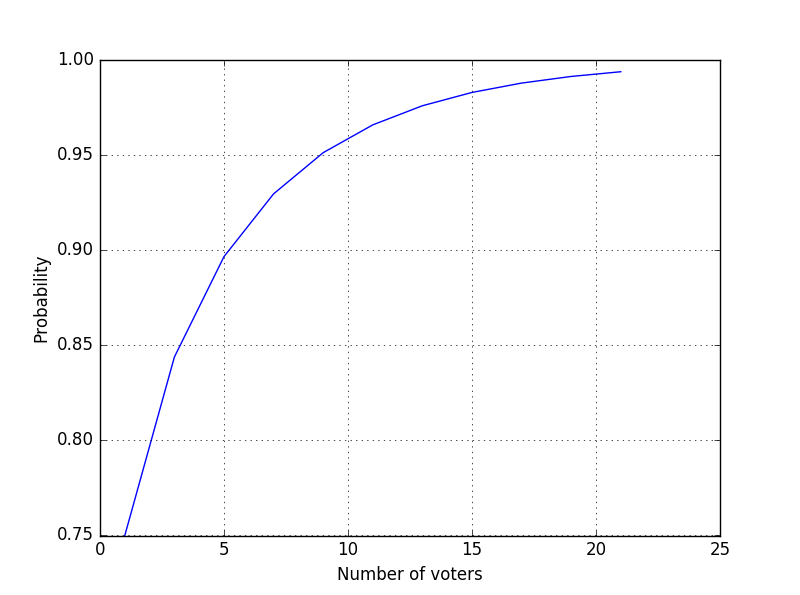
\includegraphics[width=1\textwidth]{condorcet}
\caption{The dependency between the number of voters and the probability of correct result when a single voter's accuracy is 75\%}
\end{center}
\end{figure}

Figure \ref{fig:condorcet123} shows that with a single juror's accuracy of 75\% it is required approximately 21 jurors to reach the near maximum accuracy.
\subsection{Brain-computer interface}

Brain-computer interface (BCI) is an interface that requires mental control from user to communicate with a device. It requires user to concentrate on a distinct task. Task types itself could have a large variety, for example to imagine the movement of the left hand or to stare at the picture of an animal. The interface records electroencephalographic (EEG) signals from the scalp surface which represent our brain activity. These signals have low amplitude (usually measured in microvolts), whereas frequencies above 30 Hz have especially low values which are close to zero. \cite{bci_vidal}

The signals could be translated into control commands for the external devices, what is especially useful for the people suffering from locked-in (e.g. Brainstem stroke, severe polyneuropathy) or muscle control diseases.  BCI systems could give such people a possibility to control the environment, perform word processing or even operate a neuroprosthetics or orthosis.
There are two types of BCI available: one way and two way. In case of one way type, only a computer is accepting signals from the measuring device, however a two way system deals with a bi-directional exchange of information between a computer and a measuring device. \cite{bci_shivangi}
\paragraph{}
BCI system structure could be divided into four modules \cite{bci_shivangi}:
\begin{enumerate}
\item Source Module:
This module digitizes and saves signals coming from brain without handling them. The source module component knows how to obtain data from the sensors and store them to the specifically formatted file. In addition, every recorded signal has its own labelled source, determined by the physical location of a sensor on a head. These sensor labels are stored along with the data samples, because they could be useful in the proceeding operations. 
\item Signal Processing Module:
This module is responsible for conversion of raw data signals into something more meaningful for the upcoming classification algorithm. Conversion is divided in two stages: feature extraction and feature translation. The extraction considers receiving data from the source module and preparing them for translation module, which means obtaining the signal properties, like frequency domain values for the given sensors. The feature translation is an algorithm, which determines the identity of the control signal sent with a given signal data.
\item User Application Module:
In addition to signal processing module, an application module takes the control signal to perform operations in the application. Usually the application has its own graphical interface, which allows the user to select and think about some sort of targets, like letters, images, icons or directions. The user could also give his feedback about the prediction validity through the application. The feedback could be given orally or tactilely. 
\item Operator Module:
It is a module, which defines system constants and parameters, like the length of a single concentration attempt, targets or any kind of signal processing variables. In addition, this module could contain the functionality for visualising the raw signals measured from a head or the features used in signal processing module.
\end{enumerate}
\paragraph{}
BCI use is a skill, which requires practicing. An algorithm, which translates the signal features to the control signal, should ``learn'' to output with more accuracy. Learning is performed, based on the input (target selection) provided by the user. That means, the user should participate in the algorithm teaching for many sessions. In addition, during the sessions, the user should try to concentrate in the way he usually does it. It means that if the user used to imagine a specific object or a movement to fulfil some mental task, then he/she should keep to continue to imagine the same object during all the sessions. Otherwise, such ``different thinking'' might leave a negative impact on the algorithm performance, because the signal features related to the same mental task could be way more different from each others and the classification model will not be really effective. This negative factor could be caused with a distraction experienced during the attempt or a missed focus during long-time experiments. Generally speaking, mental tasks require concentration and it takes time to get used to it.

Every prediction task is an activity considered with a subject's concentration on a mental task (target). A target could be a tangible physical object or a picture. In that case concentration on the target will most probably mean staring it. But more common is that a concentration task is done without having any visible objects, but rather by thinking or imaging the given target.

To summarize, BCI is a complex system, what has different connected layers and requires some practical skill to use it.
\subsection{Emotiv EPOC}

In order to obtain raw signal data from the brain, we use Emotiv EPOC EEG headset. It is a multi-channel wireless (communicates using Bluetooth) headset with 14 channels (sensors) for the following international locations \cite{emotiv}: AF3, F7, F3, FC5, T7, P7, O1, O2, P8, T8, FC6, F4, F8, AF4. The device converts an analog signal to digital with 14 bits resolution and 128 Hz sampling rate. The bandwith is 0.2 - 45 Hz. \cite{emotiv}

\begin{figure} [H]
\begin{center}
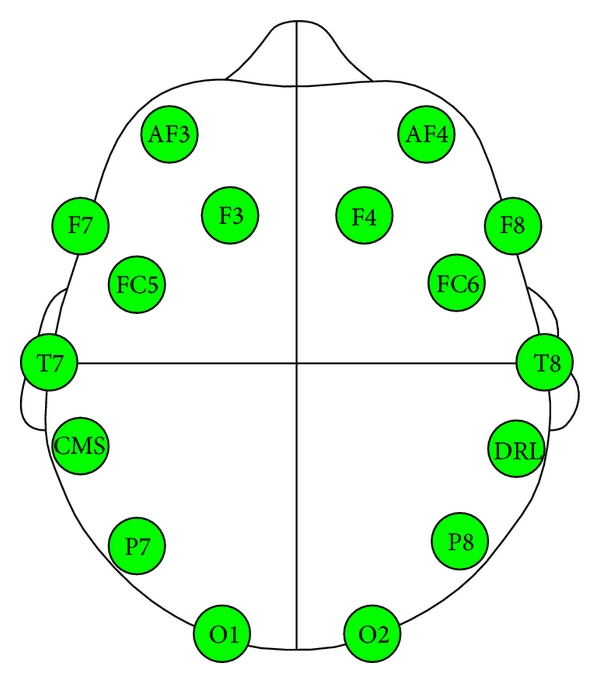
\includegraphics[width=0.7\textwidth]{emotiv_eeg}
\caption{Emotiv EEG headset sensor locations map. \cite{emotiv_eeg_pic}}
\label{fig:emotiv_eeg}
\end{center}
\end{figure}

It comes with the out of the box software Control Panel and TestBench, which visualize the signal details like signal strength timeline and already processed frequency domain values. The Control Panel software outputs recognized emotional states, facial expressions and mental commands. With TestBench it is possible to see a raw or EEG signal regarding distinct channels. In addition it provides a signal quality for the sensors and the connection status between the headset and Bluetooth receiver.

In our experiments we used the provided software only to validate the signal quality before a headset usage and data recordings. For the other purposes we wrote our custom software in order to take over the control of the signal data receiving from the headset, to handle and store it for our implementation.

\subsection{Short-time Fourier transform}

To extract the features we decompose the raw signal into subwaves. Subwaves helps to construct a frequency domain representation of the signal where frequencies and their related amplitudes are described. Although in terms of spectral analysis Fourier Transform is dominating, in case of non-stationary signals where EEG signal belongs, better to use short-time Fourier transform (STFT). \cite{alfahoum_fft}

\begin{figure} [H]
\begin{center}
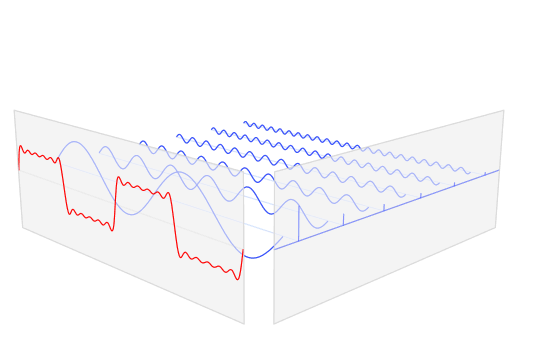
\includegraphics[width=1\textwidth]{fft}
\caption{Signal time domain conversion to frequency domain. \cite{fft} Complex signal is decomposed to sinusoids with the different frequencies and their amplitudes are used to build a frequency domain representation. }
\end{center}
\end{figure}

In STFT, a signal is split into frames of N samples each, where N is a window length. Frames overlap with some percent between each other. Before the Fourier transform a Hanning window is applied to reduce aliasing of the signal. Finally, after Fourier transform within STFT the result is outputted. It contains the spectral analysis or, in order words, the amplitudes for different frequencies.

\subsection{Classification task}

Despite the fact that relationships between some brainwaves and subject's mental states has been established, these mental states are too common and non-descriptive. For example they can help to distinguish if the subject is relaxing or concentrating on something, but more specific mental states tracking like concentrating on a certain target, a unique model should be trained for each subject. Features got from a BCI signal should be divided on groups defined by target type (i.e grouped by prediction class labels). The similarities (patterns) within the groups should be found and used to predict new input data. To define similarities a classification should be executed.

Classification is the task of learning a target function $f$ that maps each attribute set $x$ to one of the predefined class labels $y$ \cite{classification_basics}. A model received as a result of a classification could help distinguish between different target classes. Attribute set $x$(also known as features or key characteristics) could contain continuous (e.g real numbers) as well as discrete values (e.g labels).

As described above, the goal of translation phase is to understand what control signal has been described with signal features received from the extraction phase. That means we should classify our data samples, where the classes would be a set of targets a user should concentrate on. For generating a classification model a machine learning algorithm should be applied. 

A machine learning algorithm is a data-driven algorithm, that predicts in which data group a sample value belongs (classification) or which continuous output the input data maps (regression). These decisions are made based on the existing data samples which are grouped by some property. There exist two major learning types of the algorithms \cite{ml_types}:
\begin{itemize}
\item Supervised - creates a model with labeled (classified) input data samples, so that groups of data have own class label
\item Unsupervised - the algorithm does not know anything about the data as well as the classes
\end{itemize}
Unsupervised algorithm is a good way to analyse the data without knowing how to use it and on which potential groups it could be split. However, in our case we know that we should split data according to classes (targets) and thus, chose a supervised learning machine algorithm.

\subsection{Random Forest algorithm}

We will use Random Forest as a machine algorithm which is one of the most precise for the work with EEG data \cite{masso}. It shows better classification accuracy than other modern algorithms when applied on BCI signal data. 

Random Forest algorithm uses the Decision tree building algorithm, which builds the intermediate decision trees using divide-and-conquer strategy. For choosing the tree node, a heuristic is used. Heuristic is a value defined for a feature what describes how the given feature values are good at discriminating between different classes. \cite{hyper-heur}

\begin{figure} [H]
\begin{center}
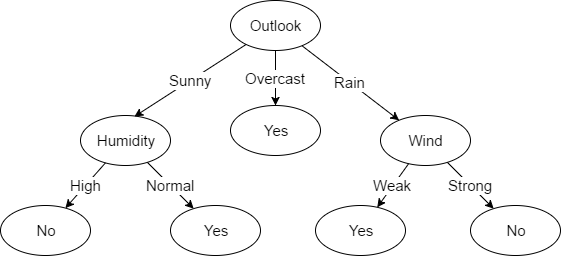
\includegraphics[width=0.7\textwidth]{decisiontree}
\caption{A sample decision tree model. It classifies whether the person will play outside for different weather conditions.}
\end{center}
\end{figure}

A Random Forest is an adaptation of Decision Tree algorithm developed by Leo Breiman and Adele Cutler, where instead of using a single tree, a bunch of trees is used. Every one of these trees is generated by using randomly selected subsets of the existing data samples and features. Finally, each tree is handled separately to find out its predicted class and using ensemble technique a final result is obtained. \cite{breiman_rf}

\subsection{Collaborative Brain-Computer Interface}

Yijun Wang {\it et.al} describes in \cite{collaborative_wang} a technique which has similar approach to this work. The main idea of their work to use collaborative EEG input data for predictions. They made a decision-making experiment using multiple users (subjects) thinking about the same targets simultaneously. Subjects must make Go (target) or NoGo (non-target) decisions in scope of their application. 

The application shows them images with animals (target) and images without animals (non-target). Each image is shown for 20ms and the subjects must make a decision if the image belongs to a target group or not.

Every subject had to train the algorithm and test it in a single user mode. Subjects managed to reach mean classification accuracy of 75.8\% with using mean response time (reaction time) 377 ms. Already this pointed on reliable prediction with single attempt usage. A collaborative classification was tried considering 5,10,15 subjects simultaneously which resulted 91.4\%, 97.6\% and 99.1\% accuracy respectively. This clearly shows improvement over the single attempt classification. 

In case of multi-user approach a weighted voting system was used, where a subject with a better prediction statistics got more weight and influenced the output result more in the future classifications. Our goal is to use multiple attempts of a single user instead of single attempt of several users as the related work tends to do. Our way is to use optimized Random Forest classification algorithm which according to \cite{masso} could bring more precise result, than support vector machine (SVM) algorithm which is used in animal classifications. Finally, a single user approach has wider fields of use and is less complex in implementation compared to the multi-user technique.

\newpage
\section{Contribution}

\subsection{Overview}
The main idea of the given work is to increase BCI accuracy sacrificing time what a user requires to concentrate on the same mental task. Thus, making BCI system more reliable if the minimum concentration time circumstance is followed. It is planned to show how the BCI with an accuracy higher than 50\% will be increased to 99\%.
The secondary idea is to show the effectiveness of a multiple attempt approach in a BCI system. 
Commonly, a regular way of prediction considers a single attempt prediction for a single user action. If there was noise in the recording due to technical issues or a subject was distracted and could not properly concentrate on the task during the attempt, then it will directly affect the classification result and dramatically reduce the accuracy. However, if we know that our system in the most cases works properly and gives the right answers, then we could compensate appearing of noisy and faulty predictions with the others with a better quality.

In multiple attempt approach the final prediction result is estimated using a majority voting over the intermediate prediction results for every attempt. Since every attempt of concentration on a task takes time (10 seconds in our case), then a drawback of the multi-attempt approach is consuming longer time than in single attempt approach. However, the accuracy should be improved in case when single attempt accuracy gives more than 50\%. Our goal is to understand how many attempts it is required to get the accuracy of 99\% in theory and check it against the reality.

\begin{figure} [H]
\begin{center}
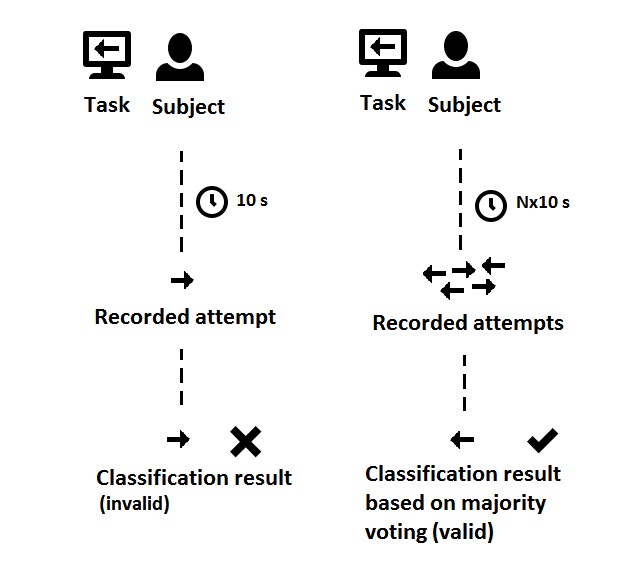
\includegraphics[height=12cm, width=1\textwidth]{main}
\caption{A main concept of multiple attempt approach. If single attempt duration is 10s and it brings only one and the final result, then applying N attempts will give several intermediate results that are combined into the final prediction using majority voting}
\label{fig:condorcet}
\end{center}
\end{figure}

\subsection{Experimental design}
To provide an experimental platform for the research question a special system was designed and implemented along with the experimental flow. The general plan is to use a two-class (two-target) BCI system to collect the data necessary for the analysis. The flow for the experiment could be described as follows:
\begin{enumerate}
\item Record the training data. This includes recording of 141 task concentration single attempts with a length of 10 second, extracting their features and storing them as a dataset along with class labels that corresponds to attempt tasks. Our purpose is to get as many samples as we can in the reasonable amount of time. It is crucial to switch between stimuli in order to get balanced training dataset.
\item Determine the baseline accuracy. That means applying machine learning techniques on the given training data. It involves training of a classifier and it's validation. Accordingly to Condorcet's jury theorem it is wise to find the method with the highest accuracy and use it as a base predictor, since this will reduce the number of samples required to obtain the target accuracy. 
\item Calculate the number of required attempts. Use Condorcet's jury theorem and the base predictor's accuracy to calculate how many attempts it is required to reach 99\% accuracy.
Upon the best baseline accuracy will be found it will be calculated how many attempts it will be required to get the desired accuracy.
\item Record the test data. Similarly to the first step it is required to measure a lot of brainwave signals and store them as a separate dataset. However, at that point the length of each session will depend on the number of attempts estimated in step 3 using Condorcet's jury theorem. Likewise in the training data collecting, it is important to keep the set balanced. Needs to be noted that the actual target labels will be stored to the dataset as well to be used in the followed accuracy calculation.
\item Analyse the multiple attempt test data. In this stage the accuracy of multiple attempt approach will be determined. The results will be observed and compared to the base predictor accuracy. The dependency between the accuracy and the number of voters will be plotted for better overview.
\end{enumerate}

Before each training or testing session a signal quality check is performed in order to ensure that the headset sensors are well placed on a head and the signal quality is high. This check is done using Emotiv Epoc Control Panel software. The training data is collected multiple times within several days which means that there is no guarantee that headset sensor locations were all the time on exactly the same place. 

Random Forest classifier is set up to use 100 trees and the random seed is manually specified in order to avoid different results within the different classification session runs. The classifier instance is set to return the probabilities of targets instead of the predicted targets. Processing continuous probabilities instead of discrete targets gives flexibility in voting systems applied in the current work.

\subsubsection{Targets}
Current system is a two-class BCI, which stands for using only two targets for concentration and prediction. For the targets in the system the following classes were selected: 
\begin{itemize}
\item Relax - the mental task is to focus sight on a fixation cross and trying to meditate.
\item Excitement - the high performance mental task where subject is focusing on a fixation cross and calculates mathematical expressions displayed on the screen.
\end{itemize}

PsychoPy \cite{psychopy} library was used for displaying the experiments window. It provides a fixation cross on the screen in order to avoid target's eyes movement, what could cause artefacts in EEG signal. The example of the graphical user interface during the measurement session is shown on Figure \ref{fig:fnCompModel}:

\begin{figure} [H]
\begin{center}
\label{fig:fnCompModel}
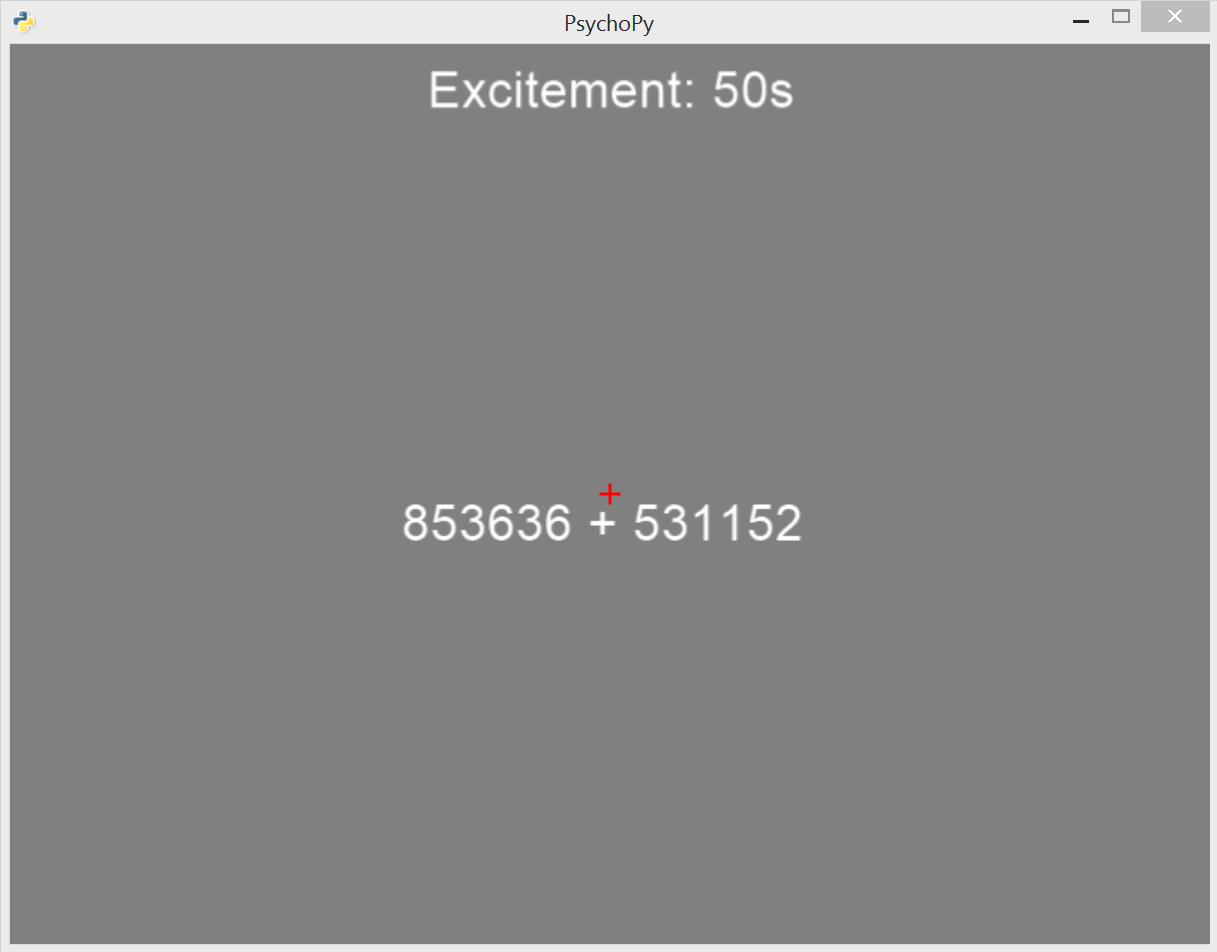
\includegraphics[width=0.8\textwidth]{test_ui}
\caption{A dialog window displaying what a subject sees during a test session for the Excitement task. A red fixation cross is located at the center of the window. Mathematical expressions are printed as an Excitement task.}
\end{center}
\end{figure}

At the very beginning of the experiments when it was not really clear what targets produce better classification results the motor activity signals were used as targets:
\begin{itemize}
\item Left - the motor task considering imaging movement of the left hand.
\item Right - the motor task considering imaging movement of the right hand.
\end{itemize}
After some constant unsuccessful (near to random) results using the motor tasks it was decided that mental task could be divided on a high and low performance types. Hence, $Excitement$ and $Relax$ targets were selected and showed better statistics.

With the several measurements and validations it was determined that 10 seconds is a suitable length for a measurement session. Taking into account that the short-time Fourier transformation extends the number of the input samples (since it uses sliding window), the single measurement session is containing 18 contains samples.

\subsection{Implementation}

For fulfilling goals in the given work a custom application was written using Python 2.7 programming language and open-source scientific libraries SciPy \cite{scipy} and NumPy \cite{numpy}. The application contains the following components:
\begin{itemize}
\item Raw data reader - connects to a BCI headset over Bluetooth and reads raw data
\item Preprocessor -  does Short-time Fourier transform of a bulk raw data and determines signal amplitudes for desired frequencies (features)
\item Data storer - stores preprocessed data to a file system (e.g CSV\footnote{Comma-Separated Values \cite{csv} file})
\item Classifier - a machine learning algorithm which teaches classifier and uses it to predict a target based on preprocessed features
\item Voting handler - it is used to handle voting to select only one prediction result among several, a detailed explanation is written in the Methods section
\end{itemize}

Some of the major components are described in the following subsections.
\begin{figure} [ht]
\begin{center}
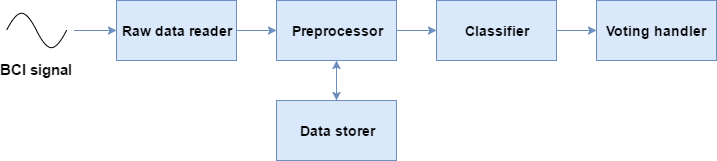
\includegraphics[width=1\textwidth]{maga_application}
\caption{The system components usage flow, while recording the test data}
\label{fig:fnCompModel}
\end{center}
\end{figure}

\subsubsection{Raw data reader}

This component is required to poll the Emotiv EPOC headset and store sent data to a temporary buffer. The communication between computer and headset is established over a Bluetooth Smart network through a USB dongle provided by the manufacturer. Emokit \cite{emokit} open-source library with minor changes is used to read the data coming to USB dongle from a headset, decrypt and encode it. Polling is done in an infinite loop. Taking into account sampling frequency of the device - 128 Hz, approximately every 8 ms a new signal is received from the headset and stored in a queue.

\subsubsection{Preprocessor}

During preprocessing a set of raw samples is converted to a frequency domain representation. To do this the Short Time Fourier Transform is used with a sliding window. Sliding window technique allows to capture more precisely non-constant signals. Sliding window length equals to 1 s with 0.5 s overlapping. These factors increase the number of samples to $2*N-2$ where $N$ is the original number of samples. For example a BCI session with a duration of 1 minute will output 119 samples.

According to Emotiv EPOC specifications \cite{emotiv} 45 Hz is the maximum bandwidth value for the signal. In our implementation we use 1 -- 45 Hz for the frequency range. An example plot of obtained frequency domain values is shown in Appendix \ref{app:1}.

\subsubsection{Data storer}

This component is responsible for data recording into CSV files after the run of brain signal measurement sessions and applying preprocessing. Training and test data are recorded into separate files. Each row in a CSV file corresponds to a sample. A sample contains amplitude values for frequencies from 1--45 Hz for each sensor what makes in total 630 values for a sample. 

\subsubsection{Classifier}

Classifier component is responsible for determining a target (class) from the number of samples given by preprocessor component. Each sample (record) contains 630 features. This records compose a dataset which is fed up to a classifier (machine learning algorithm) to train it. 

A 5-fold cross-validation is done in the current component. Technically this means selecting proportional validation data chunks (with a size of 20\% of the training dataset) from the whole dataset without overlapping and using the rest of the samples as training data. This will result in training several classifiers. These classifiers prediction outputs will be concatenated and used further as a training data prediction.

Instead of discrete class prediction labels what could be returned by Random Forest (RF), we rather ask RF to return the probabilities for the labels to be predicted. It gives us flexibility to apply various techniques described in the subsequent section. RF is set up to use 100 trees, what was considered as the optimal number to obtain precise prediction results with reasonable time.

\newpage
\section{Methods} \label{methods}

The given section describes different techniques (predictors) what are used to determine one single prediction result at the different classification levels:
\begin{itemize}
\item Sample classification level - at this level a prediction class is being estimated for a single sample based on the class probabilities returned with a Random Forest classifier. A sample-based action predictor is used to do this.
\item Attempt classification level - at this level a prediction class is being estimated based on multiple sample classes, which all belong to one concentration attempt. A voting-based action predictor  is used to do this.
\item Multi-attempt classification level - at this level a prediction class is being estimated based on the classes estimated at a attempt classification level, where all concentration attempts belong to the same task (i.e concentration on one mental task using multiple attempts). A majority voting is applied at this level to estimate the prediction class.
\end{itemize}

\subsection{Sample-based action predictor}

This predictor is used to determine what class label should be correspond to a given RF class probability. It is called sample-based because it decides what prediction result should be for one sample (i.e sample level prediction). To make the sample-based prediction we are using so-called \textit{probability threshold predictors} which are described as in Definition \ref{def:prb_thr}.
\theoremstyle{definition}
\begin{definition}
\label{def:prb_thr}
Probability threshold predictor is a method for classifying a sample using class probability estimated with Random Forest algorithm, where one of the prediction classes could be selected only if it has probability higher than the probability threshold. 
\end{definition}
In this work we will use two different types of probability thresholds described subsequently. 
\subsubsection{\sfrac{1}{2}-probability threshold}
This is a probability threshold of 50\% in two-class system. Using it, the class will be selected if its probability estimated by RF exceeds 50\% or \sfrac{1}{2}.
\subsubsection{$T$-probability threshold}
For the given approach we dynamically calculate threshold $T$ for one distinct class. If RF estimated probability for this class exceeds $T$, then this class will be the result of the prediction, otherwise - the second. To find $T$ we set up different predictors with different thresholds in a range of 0-100\% with a step of 1\%. We compare the accuracies of these predictors and take one with the highest to use its threshold as $T$.

\subsection{Voting-based action predictor}
A single user concentration attempt lasts for 10 seconds, which produces 18 samples in total. After applying a sample-based predictor we will get 18 classes, each for one sample. To convert these 18 classes to a single answer (i.e find the prediction answer at the concentration attempt level) a voting-based action predictor is used. This predictor is used to vote for a prediction result based on the 18 classes. The following subsections describe the two variants of voting-based predictors.

\subsubsection{Majority voting}

This is a rather simple way -- a class is selected as final prediction for the concentration attempt if it appears in the input set more than the other class. 

\subsubsection{Decision threshold voting}
In this case the voting result depends on whether the number of occurrences for the class exceeds the minimum threshold value. The threshold is chosen dynamically by trying out all available values from 1 to 18 with a step of 1 and measuring the final two-class accuracy to determine the best. 

\theoremstyle{definition}
\begin{definition}
Decision threshold voting is a method of estimating a final prediction result class from the given set of classes, where one of the prediction result classes could be selected only if it appears in the given set more times than is the number of threshold.
\end{definition}

\subsection{Action prediction based on multiple attempts}
In case of multiple attempt approach majority voting  is applied to the prediction results of individual attempts. For example, if a user should concentrate on a mental task for 5 attempts in a row, then as a result of applying sample-based and voting-based predictors there will be 5 classes -- each corresponds to a single attempt. To estimate a single class from them majority voting is used.

To fulfil this approach and see how we can actually increase the accuracy of a BCI system we:
\begin{enumerate}
\item tried out different sample-based and voting-based predictors to estimate the single concentration attempt accuracies (baseline accuracies),
\item using Condorcet's jury theorem and the baseline accuracies calculated the minimum number of concentration attempts required to reach accuracy of 99\% for each predictor,
\item based on the previous step, selected the minimum number of concentration attempts required and carried out test data measurement according to the new length of concentration task,
\item used some of the predictors with the best accuracies, got their empirical classification accuracies for the multi-attempt approach and compared them to the results estimated by Condorcet's jury theorem.
\end{enumerate}

\newpage
\section{Experimental Results}

The experimentally obtained accuracies for the single and multiple attempt approaches are described in the followed subsections. Finally, multiple attempt approach results are compared to the theoretical objections using different high-accuracy predictors.

\subsection{Single attempt approach}

In this section we describe the accuracies for single attempt approach using different predictors for different levels: sample classification (estimating a class for a single sample) and attempt classification (estimating a class for prediction classes on one concentration attempt). Table \ref{tab:table1} summarizes the techniques that we use in the single attempt approach. 
\begin{table}[H]
\begin{center}
  \begin{tabular}{ | c | c | c | c | }
    \hline
    \textbf{Sample classification} & \textbf{Attempt classification} \\ \hline
    \sfrac{1}{2}-probability threshold & Majority voting \\ \hline
	$T$-probability threshold & Decision threshold voting\\ \hline
  \end{tabular}
\end{center}
\caption{Classification techniques used for different levels: sample classification and attempt classification.} \label{tab:table1} 
\end{table}
We also tried to calculate the prediction accuracy without using voting, that means that samples were not grouped together by their concentration attempt before finding the final accuracy. We tried to use all of the combinations of the predictors mixing up together different sample classification and attempt classification techniques. That gave us 6 different approaches in total including the sample classification techniques without voting. The following subsections are split into these 6 different techniques.

\subsubsection{Sample classification without voting approach}\label{no-voting}

In this approach only sample-based predictors are used, without using any of the voting techniques. Single sample classes are predicted (using \sfrac{1}{2}-probability threshold or $T$-probability threshold) and the average accuracy is measured among them. 

\paragraph{\sfrac{1}{2}-probability threshold}~\\

The average prediction accuracy on the test data is determined as \textbf{67.1\%}. Based on the prediction results the following confusion matrix is constructed:
\begin{table}[H]
 \label{tab:title} 
\begin{center}
  \begin{tabular}{ | c | c | c | c | }
    \hline
     & Predicted Relax & Predicted Excitement & Total \\ \hline
    Actually Relax & 597 & 570 & 1167 \\ \hline
    Actually Excitement & 263 & 1105 & 1368 \\ \hline
    Total & 860 & 1675 & 2535 \\ 
    \hline
  \end{tabular}
\end{center}
\caption{Confusion matrix showing classifier's prediction performance using \sfrac{1}{2}-probability threshold without voting. The accuracy is 67.1\%.}
\end{table}

This table shows that $Excitement$ is better recognized and has approximately 0.24 error rate, meanwhile the target $Relax$ has almost 50\% accuracy.

\paragraph{$T$-probability threshold}~\\

This technique is used in order to balance the prediction accuracies between the classes. Threshold or the minimum probability for the most frequent class is set up as a border between the two classes. Threshold is compared to the labels probabilities returned by Random Forest, which are calculated inside the algorithm's implementation. 

Since the $Excitement$ is the class, which appears more times in prediction results than $Relax$ and has higher prediction accuracy, it is suitable candidate to have the minimum probability threshold, what is higher than 50\%. The dependency between different probability thresholds for the $Excitement$ and the prediction accuracies for the training data is shown on the Figure \ref{fig:probability_thresholds}.
\begin{figure} [H]
\begin{center}
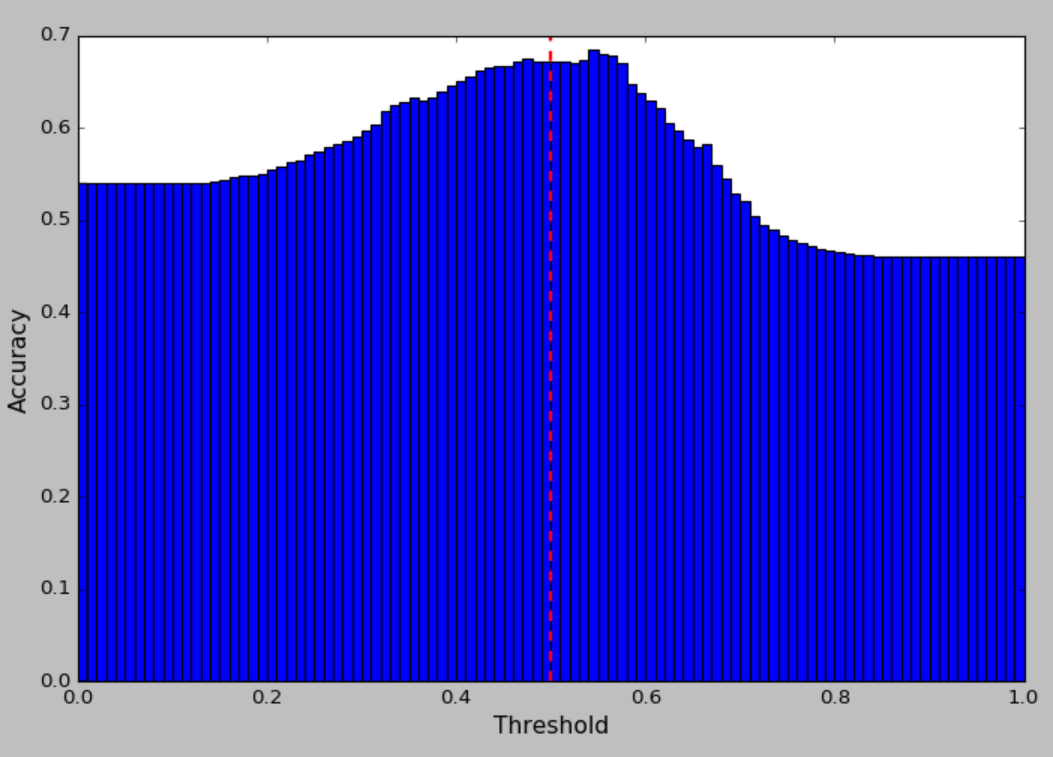
\includegraphics[width=1\textwidth]{probability_thresholds}
\caption{Training data prediction accuracy dependency on the Excitement probability threshold value.}
\label{fig:probability_thresholds}
\end{center}
\end{figure}

Comparing the prediction accuracies using different thresholds and selecting the best combination gives the probability threshold 0.54 ($T$=0.54) for the $Excitement$ class. The given $T$ is used in all subsequent $T$-probability threshold predictors. Below is the confusion matrix for the given approach. The prediction accuracy is \textbf{68.4\%}.

\begin{table}[H]
\begin{center}
  \begin{tabular}{ | c | c | c | c | }
    \hline
     & Predicted Relax & Predicted Excitement & Total \\ \hline
    Actually Relax & 754 & 413 & 1167 \\ \hline
    Actually Excitement & 387 & 981 & 1368 \\ \hline
    Total & 1141 & 1394 & 2535 \\ 
    \hline
  \end{tabular}
\end{center}
\caption{Confusion matrix showing classifier's prediction performance using $T$-probability threshold without voting, where $T$ for $Excitement$ is 0.54. The accuracy is 68.4\%.} \label{tab:title} 
\end{table}

\subsubsection{Majority voting}

In the following technique a majority voting is applied to 18 prediction samples, which belong to one concentration attempt. After the voting, only a single class is estimated from each group of 18 samples (the one which appears more times) which corresponds to the prediction result of the given attempt. Different sample-based predictors are used to determine the labels of individual samples.

\paragraph{\sfrac{1}{2}-probability threshold}~\\

Finding the average accuracy using \sfrac{1}{2}-probability threshold and majority voting gives the accuracy of \textbf{78.5\%}.
\begin{table}[H]
\begin{center}
  \begin{tabular}{ | c | c | c | c | }
    \hline
     & Predicted Relax & Predicted Excitement & Total \\ \hline
    Actually Relax & 37 & 27 & 64 \\ \hline
    Actually Excitement & 3 & 73 & 76 \\ \hline
    Total & 40 & 100 & 140 \\ 
    \hline
  \end{tabular}
\end{center}
\caption{Confusion matrix showing classifier's prediction performance using \sfrac{1}{2}-probability threshold with majority voting. The accuracy is 78.5\%.} 
\end{table}

\paragraph{$T$-probability threshold}~\\

Using the $T$ threshold ($T$=0.54) that was determined in the Section \ref{no-voting} for the $Excitement$ target, the prediction accuracy is \textbf{83.6\%}.

\begin{table}[H]
\begin{center}
  \begin{tabular}{ | c | c | c | c | }
    \hline
     & Predicted Relax & Predicted Excitement & Total \\ \hline
    Actually Relax & 49 & 15 & 64 \\ \hline
    Actually Excitement & 8 & 68 & 76 \\ \hline
    Total & 57 & 83 & 140 \\ 
    \hline
  \end{tabular}
\end{center}
\caption{Confusion matrix showing classifier's prediction performance using $T$-probability threshold with majority voting, where $T$ for $Excitement$ is 0.54. The accuracy is 83.6\%.} 
\end{table}

\subsubsection{Decision threshold voting}

The following approach is based on calculating the voting threshold which brings the highest accuracy. The decision threshold is defined as the minimum number of occurrences of a class in a series of attempts to make this class win in a vote. In our case a threshold is applied to the $Excitement$ class, since it is a high-accuracy class. The dependency between the threshold value and the accuracy is shown on Figure \ref{fig:fnCompModel}.

\begin{figure} [H]
\begin{center}
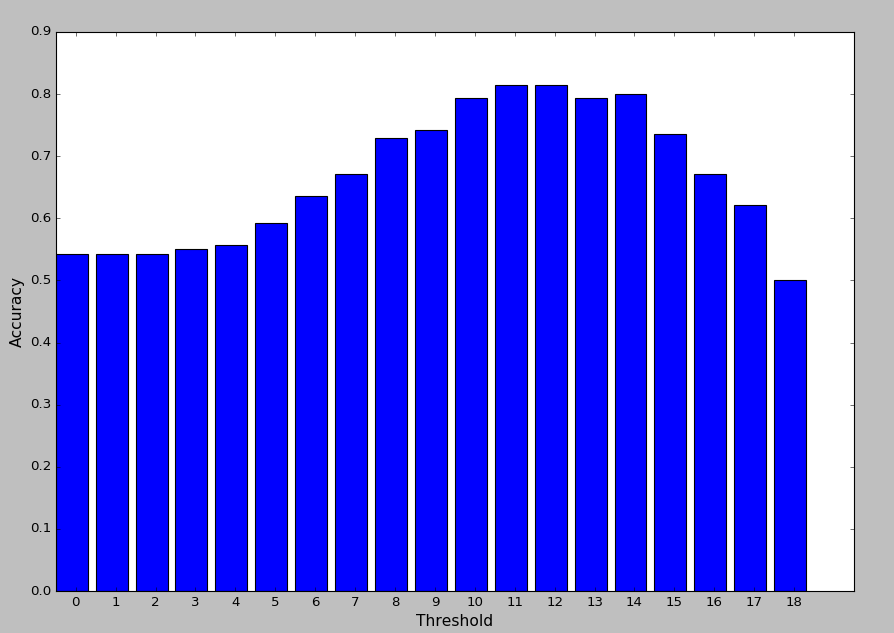
\includegraphics[width=1\textwidth]{threshold_accuracy_curve}
\caption{Prediction accuracy dependency on the Excitement threshold value}
\label{fig:fnCompModel}
\end{center}
\end{figure}

According to the plot, the threshold for a voting for $Excitement$ with the best classification accuracy are 11 and 12. In our implementation we take the first value, which is 11.

\paragraph{\sfrac{1}{2}-probability threshold}~\\

Using the \sfrac{1}{2}-probability threshold to determine the single sample's class and subsequently applying decision threshold to determine single concentration attempt's class gives the accuracy of \textbf{81.4\%}.
\begin{table}[H]
\begin{center}
  \begin{tabular}{ | c | c | c | c | }
    \hline
     & Predicted Relax & Predicted Excitement & Total \\ \hline
    Actually Relax & 45 & 19 & 64 \\ \hline
    Actually Excitement & 7 & 69 & 76 \\ \hline
    Total & 52 & 88 & 140 \\ 
    \hline
  \end{tabular}
\end{center}
\caption{Confusion matrix showing classifier's prediction performance using \sfrac{1}{2}-probability threshold with decision threshold voting, where decision threshold for $Excitement$ is 11. The accuracy is 81.4\%.} 
\end{table}

Usage of decision threshold has balanced false negatives and true negatives, however the error rate for the $Excitement$ has grown compared to the majority voting strategy.

\paragraph{$T$-probability threshold}~\\

This approach uses $T$-probability threshold to estimate a class for a single sample. $T$ is defined before as 0.54 for the $Excitement$ class. Applying decision threshold voting after the given sample-based predictor gives the accuracy of \textbf{81.4\%}.

\begin{table}[H]
\begin{center}
  \begin{tabular}{ | c | c | c | c | }
    \hline
     & Predicted Relax & Predicted Excitement & Total \\ \hline
    Actually Relax & 53 & 11 & 64 \\ \hline
    Actually Excitement & 15 & 61 & 76 \\ \hline
    Total & 68 & 72 & 140 \\ 
    \hline
  \end{tabular}
\end{center}
\caption{Confusion matrix showing classifier's prediction performance using $T$-probability threshold with decision threshold voting, where decision threshold for $Excitement$ is 11 and $T$ for $Excitement$ is 0.54. The accuracy is 81.4\%.} 
\end{table}

Despite that this approach gives different values in confusion matrix from the \sfrac{1}{2}-probability threshold predictor using the same voting technique, their accuracies are equal.

\subsection{Multiple attempt approach}

In this section we describe what are the estimated and actual accuracy results for multiple attempt approach. During the estimations single attempt accuracies are used.
\subsubsection{Condorcet's jury theorietical estimation}\label{condorcet1}
Based on the predictors accuracy results for single attempt approach we define how many attempts it is required to reach the minimum accuracy of 99\%. Using Condorcet's jury theorem we have calculated the number of required attempts and composed the following comparative table. The table is ordered by the prediction values of the accuracies:

\begin{table}[H]
\label{tab:title} 
\begin{center}
  \begin{tabular}{ | l | c | c | c | }
    \hline
    Method & \parbox[c]{1.8cm}{\raggedright Single attempt accuracy (\%)} &\parbox[c]{1.8cm}{\raggedright Attempts required}\\ \hline
    $T$-probability threshold with majority voting & 83.6 & 9 \\ \hline
    \sfrac{1}{2}-probability threshold with decision threshold voting & 81.4 & 11 \\ \hline
	$T$-probability threshold with decision threshold voting & 81.4 & 11 \\ \hline
	\sfrac{1}{2}-probability threshold with majority voting & 78.6 & 15 \\ \hline
    $T$-probability threshold without voting & 68.4 & 37\\ \hline
    \sfrac{1}{2}-probability threshold without voting & 67.1 & 43\\ \hline
  \end{tabular}
\end{center}
\caption{Different predictor accuracies and the required number of attempts to get to 99\% accuracy.}
\end{table}

According to the given results the $T$-probability threshold with majority voting is the best among the methods and it requires only 9 measurement attempts for a single concentration task to get the desired accuracy. We use this number of attempts in the subsequent multiple attempt approach to measure the performance on test data.

\begin{figure} [H]
\begin{center}
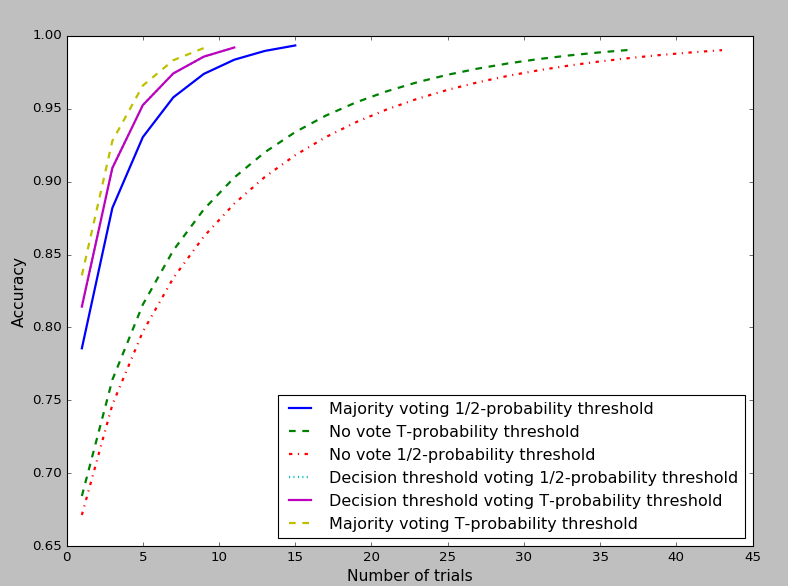
\includegraphics[width=1\textwidth]{condorcet_dependency_training}
\caption{Theoretical estimate of the number of attempts and the expected accuracy for different predictors. Note: \sfrac{1}{2}-probability threshold with decision threshold voting is overlapping with $T$-probability threshold with decision threshold voting.}
\label{fig:fnCompModel}
\end{center}
\end{figure}

Along with $T$-probability threshold with majority voting predictor, we estimate the prediction accuracies for the other top 3 methods to compare their empirical results as well. Since they should have different accuracies for 9 attempts, we define the following table, where the expected accuracies for 9 attempts are defined.

\begin{table}[H]
\label{tab:title} 
\begin{center}
  \begin{tabular}{ | l | c | c | c | }
    \hline
    Method &\parbox[c]{1.8cm}{\raggedright Accuracy for 9 attempts (\%)}\\ \hline
    $T$-probability threshold with majority voting & 99.6 \\ \hline
    \sfrac{1}{2}-probability threshold with decision threshold voting & 98.6 \\ \hline
	$T$-probability threshold with decision threshold voting & 98.6 \\ \hline
	\sfrac{1}{2}-probability threshold with majority voting & 97.4 \\ \hline
  \end{tabular}
\end{center}
\caption{Different predictor's expected accuracies in 9 attempts approach.}
\end{table}

\subsubsection{Condorcet's jury empirical results}

We have selected the lowest number of attempts: 9 -- it was calculated with Condorcet's jury theorem and theoretically should be enough to produce 99\% accuracy for $T$-probability threshold with majority voting predictor. According to that number we run brain signal measurement sessions to record the test data, where each concentration task requires 9 attempts (i.e it is 9 times longer than single attempt of concentration task).

After the test data recording we applied a predictor to each attempt separately to get the 9 classes. To get the final class from 9 classes, we use majority voting. In this work we calculated the actual prediction accuracies for the 4 best predictors and their results are described in the followed paragraphs.

\paragraph{$T$-probability threshold with majority voting}~\\

The given approach has the prediction accuracy of \textbf{88.1\%}.  
\begin{table}[H]
\begin{center}
  \begin{tabular}{ | c | c | c | c | }
    \hline
     & Predicted Relax & Predicted Excitement & Total \\ \hline
    Actually Relax & 16 & 5 & 21 \\ \hline
    Actually Excitement & 0 & 21 & 21 \\ \hline
    Total & 16 & 26 & 42 \\ 
    \hline
  \end{tabular}
\end{center}
\caption{Confusion matrix showing classifier's prediction performance using $T$-probability threshold with majority voting predictor in 9 attempt approach. The accuracy is 88.1\%.} 
\end{table}

\paragraph{\sfrac{1}{2}-probability threshold with decision threshold voting}~\\

The given approach has the prediction accuracy of \textbf{90.5\%}.  
\begin{table}[H]
\begin{center}
  \begin{tabular}{ | c | c | c | c | }
    \hline
     & Predicted Relax & Predicted Excitement & Total \\ \hline
    Actually Relax & 17 & 4 & 21 \\ \hline
    Actually Excitement & 0 & 21 & 21 \\ \hline
    Total & 17 & 25 & 42 \\ 
    \hline
  \end{tabular}
\end{center}
\caption{Confusion matrix showing classifier's prediction performance using \sfrac{1}{2}-probability threshold with decision threshold voting predictor in 9 attempt approach. The accuracy is 90.5\%.} 
\end{table}

\paragraph{$T$-probability threshold with decision threshold voting}~\\

The given approach has the prediction accuracy of \textbf{95.2\%}.  
\begin{table}[H]
\begin{center}
  \begin{tabular}{ | c | c | c | c | }
    \hline
     & Predicted Relax & Predicted Excitement & Total \\ \hline
    Actually Relax & 21 & 0 & 21 \\ \hline
    Actually Excitement & 2 & 19 & 21 \\ \hline
    Total & 23 & 19 & 42 \\ 
    \hline
  \end{tabular}
\end{center}
\caption{Confusion matrix showing classifier's prediction performance using $T$-probability threshold with decision threshold voting predictor in 9 attempt approach. The accuracy is 95.2\%. Note that out of 42 task attempts only 2 were misclassified.}
\end{table}

\paragraph{\sfrac{1}{2}-probability threshold with majority voting}~\\

The given approach has the prediction accuracy of \textbf{76.2\%}.  
\begin{table}[H]
\begin{center}
  \begin{tabular}{ | c | c | c | c | }
    \hline
     & Predicted Relax & Predicted Excitement & Total \\ \hline
    Actually Relax & 11 & 10 & 21 \\ \hline
    Actually Excitement & 0 & 21 & 21 \\ \hline
    Total & 11 & 31 & 42 \\ 
    \hline
  \end{tabular}
\end{center}
\caption{Confusion matrix showing classifier's prediction performance using \sfrac{1}{2}-probability threshold with majority voting predictor in 9 attempt approach. The accuracy is 76.2\%.} 
\end{table}

\subsubsection{Theoretical and empirical results comparison}

To compare the theoretical and empirical results for the prediction accuracies based on 9 attempts the following table is built:
\begin{table}[H]
\begin{center}
  \begin{tabular}{ | l | c | c | c | }
    \hline
    Method &\parbox[c]{1.8cm}{\raggedright Expected accuracy for 9 attempts (\%)} &\parbox[c]{1.8cm}{\raggedright Actual accuracy for 9 attempts (\%)} &\parbox[c]{1.8cm}{\raggedright Difference (\%)}\\ \hline
    \parbox[c]{7cm}{\raggedright $T$-probability threshold with majority voting} & 99.6 & 88.1 & 11.5 \\ \hline
    \parbox[c]{7cm}{\sfrac{1}{2}-probability threshold with decision threshold voting} & 98.6 & 90.5 & 8.1 \\ \hline
	\parbox[c]{7cm}{$T$-probability threshold with decision threshold voting} & 98.6 & \textbf{95.2} & 3.4\\ \hline
	\parbox[c]{7cm}{\sfrac{1}{2}-probability threshold with majority voting} & 97.4 & 76.2 & 21.2\\ \hline
  \end{tabular}
\end{center}
\caption{Expected and actual prediction accuracies for 9 attempt approach. Ordered by the expected accuracy values.}
\end{table}

It can be seen, that all the methods have the accuracy lower than the expected theoretical estimate. The predictor that expected to get 99\% of accuracy ($T$-probability threshold with majority voting) got actually 88.1\% which is 11.5\% lower than the expected. The $T$-probability threshold with decision threshold voting predictor has the lowest difference from the expected accuracy -- 3.4\%. In addition, this method has the highest prediction accuracy -- 95.2\%, what makes it more reliable than others. According to the results, the methods which use decision threshold voting have lower difference between the expected and actual results.

From these we conclude that repeating classification attempts using imperfect classifier does indeed improve the overall classification accuracy and can be considered as a path towards reliable BCI.

\newpage
\section*{Conclusion}
\addcontentsline{toc}{section}{Conclusion}

Nowadays BCI system performance is mostly measured with a prediction accuracy. State of the art prediction accuracies of modern BCIs are far from optimal and this prevents us from having reliable BCI systems. Reliability is a key factor for the most of the technological or medical industries, that means that current BCI systems are not suitable for most of the practical applications. The approach proposed in this work could leverage using time as a measure of performance instead of accuracy. Unlike former BCI systems, the multi-attempt approach does not have meaningful limitations in prediction accuracy. Their accuracy could be always more than 99.9\%, what is high enough to  provide their spread to different industries and our daily life. However, that means that BCI systems will provide their own time requirements, what should fit into the business side's limitations. On the other hand, the given approach allows flexibility in the time sacrificing and accuracy selection -- users could regulate BCI performance with the time they apply to a concentration on a mental task.

In order to make all this available it is required for each BCI system to provide its time/accuracy dependency model what will describe how the accuracy will be improved within applied time. 


\paragraph{Limitations}~\\

The first major limitation for this work is the number of the attempts used in multi-attempt approach. Since concentration on a mental task is not really simple activity (especially on $Excitement$) and it requires 10 seconds of concentrating per each attempt, we used only 9 attempts, which is the smallest for the provided predictors. As the experimental results show with 9 attempts we were able to get only 95.2\% for the highest accuracy, which is lower on 3.8\% than our initial goal.

Training and test data amount could be higher. In total we have measured 42 multi-attempt concentrations, what corresponds to the same number of classification results for multi-attempt approach. This number is used to calculate the average prediction accuracy of multi-attempt solution, what is obviously too small.
Another limitation is considering the training data, where we are using only 2535 samples. Increase of this number should positively influence on the classifier's performance and thus it could be expected that test data would be predicted better.

All the BCI recordings were done on the author of the thesis, that means that only one person was participating in the mental experiments. The accuracy numbers obtained for single and multiple attempt approaches could be different if the subject would be another person. It would be more precise to carry out these experiments on group of subjects and take their average results as final.

\paragraph{Future work}~\\

Considering that we did not reach our goal accuracy of 99\% in multi-attempt approach, it would be reasonable to try running in such a mode where the user has to repeat the attempts for as long as it takes to reach 99\% accuracy. Once this mode is implemented we will run the experiments on multiple test subjects to estimate the number of attempts and time per action required to reach 99\% accuracy.

\newpage
\input{maga-bbl.bbl}
\bibliographystyle{unsrt}
\bibliography{maga-bbl}

\newpage

\section*{Appendix A: Visualization of the signal in frequency space}
\addcontentsline{toc}{section}{Appendix A}
\label{app:1}
\begin{figure} [H]
\begin{center}
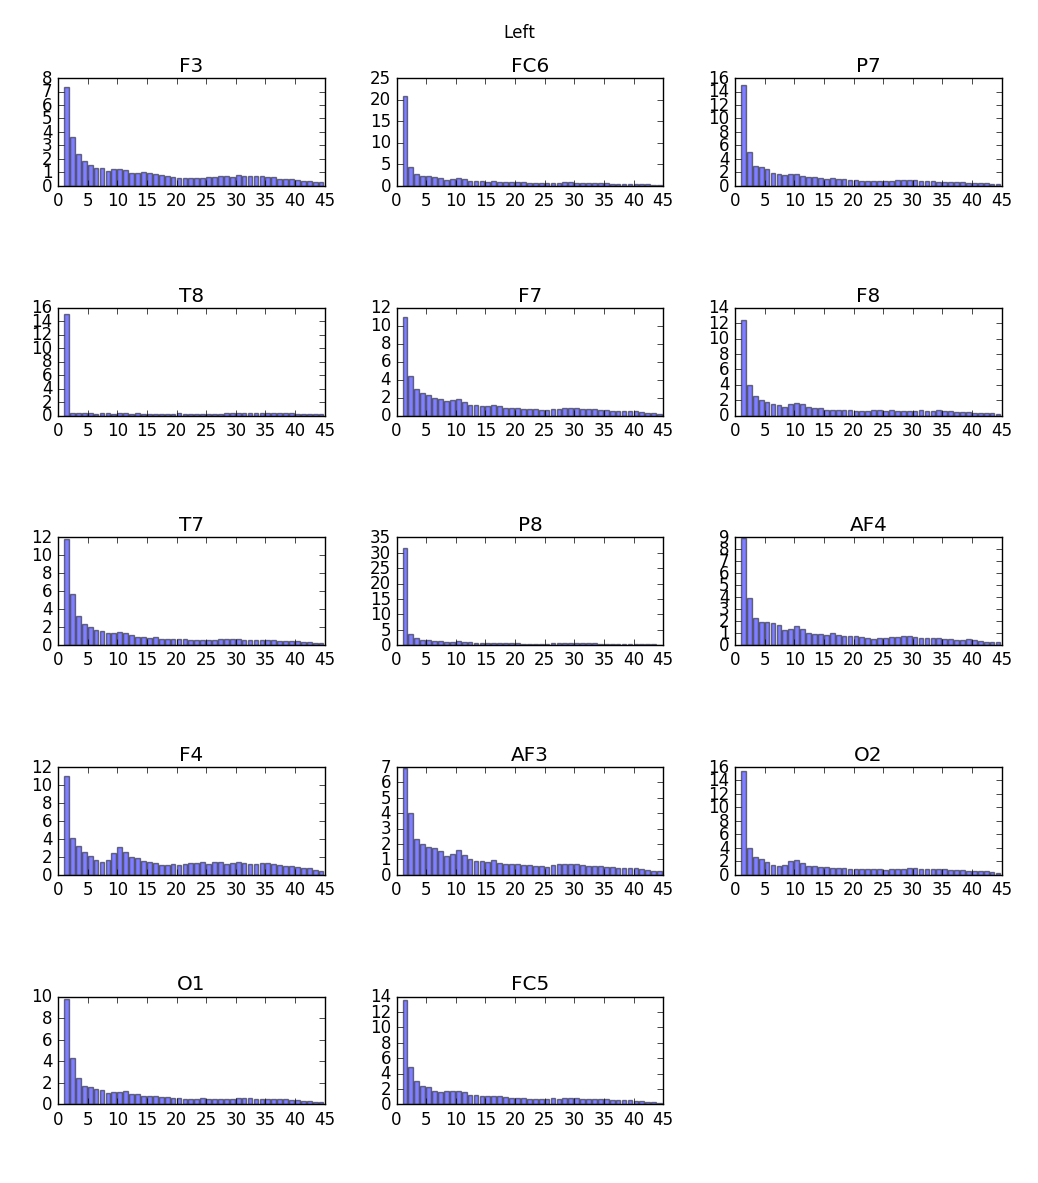
\includegraphics[width=1\textwidth]{left_amplitudes}
\caption{A sample frequency domain plot for a signal from concentration on ``Left'' mental task. Horizontal axis is measured in Hz. Vertical in $\mu$V.}
\end{center}
\end{figure}

\newpage
\section*{Appendix B: Source code repository URL}
The source code for the given implementation is stored in GitHub public repository:
\url{https://github.com/jevgeniS}
\addcontentsline{toc}{section}{Appendix B}

\pagebreak
\section*{\small Non-exclusive licence to reproduce thesis and make thesis public}


I, Jevgeni Savostkin (date of birth: 13th of March 1990),

\begin{tabbing}
\= Xiii\=\kill
\>1. \> herewith grant the University of Tartu a free permit (non-exclusive licence) to:\\\\ 

\>1.1\> 
\begin{minipage}[t]{14.2cm}
reproduce, for the purpose of preservation and making available to the public, including for addition to the DSpace digital archives until expiry of the term of validity of the copyright, and
\end{minipage}
\\\\
\>1.2 
\begin{minipage}[t]{14.2cm}
make available to the public via the web environment of the University of Tartu, including via the DSpace digital archives until expiry of the term of validity of the copyright,\\ 

Towards Reliable Brain-Computer Interface: Achieving Perfect Accuracy by Sacrificing Time\\   

supervised by Ilya Kuzovkin and Raul Vicente

\end{minipage}\\\\ 
\>2. \>I am aware of the fact that the author retains these rights.\\\\
\>3. \>
\begin{minipage}[t]{14.2cm}
I certify that granting the non-exclusive licence does not infringe the intellectual property rights or rights arising from the Personal Data Protection Act. 
\end{minipage}\\
\end{tabbing}

\noindent
Tartu, 18.05.2017


\end{document}
